\documentclass[paper=a4, fontsize=11pt]{scrartcl}

\usepackage{fancyhdr}
\pagestyle{fancyplain}
\setlength{\headheight}{25pt}
\renewcommand{\headrulewidth}{0pt}
\renewcommand{\footrulewidth}{0pt}
\usepackage{graphicx}
\usepackage{epigraph}
\usepackage{amsmath,amssymb,amsfonts }
\usepackage{lastpage}
\usepackage{algorithm}
\usepackage{algpseudocode}


\newcommand{\Abf}{\ensuremath{\mathbf{A}}}
\newcommand{\bbf}{\ensuremath{\mathbf{b}}}
\newcommand{\cbf}{\ensuremath{\mathbf{c}}}
\newcommand{\abf}{\ensuremath{\mathbf{a}}}
\newcommand{\xbf}{\ensuremath{\mathbf{x}}}
\newcommand{\ybf}{\ensuremath{\mathbf{y}}}
\newcommand{\Rbb}{\ensuremath{\mathbb{R}}}
\newcommand{\Rbf}{\ensuremath{\mathbf{R}}}
\newcommand{\fo}{\ensuremath{f_0}}
\newcommand{\fii}{\ensuremath{f_i}}
\newcommand{\transpose}[1]{#1^\mathsf{T}}
\newcommand{\norm}[1]{\ensuremath{\lVert{#1}\rVert}}


\newtheorem{definition}{Definition}[section]
\newtheorem{theorem}{Theorem}[section]
\newtheorem{lemma}[theorem]{Lemma}
\newtheorem{proposition}[theorem]{Proposition}
\newtheorem{corollary}[theorem]{Corollary}
\newtheorem{observation}[theorem]{Observation}

\newenvironment{proof}[1][Proof]{\begin{trivlist}
\item[\hskip \labelsep {\bfseries #1}]}{\end{trivlist}}
%\newenvironment{definition}[1][Definition]{\begin{trivlist}
%\item[\hskip \labelsep {\bfseries #1}]}{\end{trivlist}}
\newenvironment{example}[1][Example]{\begin{trivlist}
\item[\hskip \labelsep {\bfseries #1}]}{\end{trivlist}}
\newenvironment{remark}[1][Remark]{\begin{trivlist}
\item[\hskip \labelsep {\bfseries #1}]}{\end{trivlist}}

\newcommand{\qed}{\nobreak \ifvmode \relax \else
      \ifdim\lastskip<1.5em \hskip-\lastskip
      \hskip1.5em plus0em minus0.5em \fi \nobreak
      \vrule height0.75em width0.5em depth0.25em\fi}


\newcommand{\lecture}{Assignment \#3 Report} %lecture number and date goes here
\newcommand{\lecturedate}{March 3, 2016} %lecture date goeshere
\newcommand{\scribe}{Michael Lam} %student name goes here

\fancyhead[L]{\small Winter 2016}
\fancyhead[R]{\small \lecture}
%\fancyfoot[L]{\small CS 519-006: Deep Learning}
%\fancyfoot[C]{}
\fancyfoot[C]{\thepage\ of \pageref{LastPage}}


\begin{document}


\newcommand{\horrule}[1]{\rule{\linewidth}{#1}} % Create horizontal rule command with 1 argument of height

\title{	
\normalfont \normalsize
\vspace{-30pt}
\textsc{CS 519-006: Deep Learning} \\ [10pt]
\horrule{0.5pt} \\[0.4cm] % Thin top horizontal rule
\LARGE \lecture\\ % The assignment title
\vspace{5pt}
\normalsize \scribe\\
\lecturedate\\
\horrule{2pt} \\[0.5cm] % Thick bottom horizontal rule
}


\date{} % Today's date or a custom date

\maketitle
\vspace{-100pt}
%\epigraph{''Every problem is an optimization problem in disguise.''}{--Anonymous}

\begin{abstract}
This assignment explores tuning a convolutional neural network using Keras. We investigate various tuning methodologies and report the results.
\end{abstract}

\section{Question 1}

{\small Remove the dropout layer after the fully-connected layer (5 points). Save the model after training.}\\

We removed the dropout layer after the fully-connected layer.  Figure \ref{fig:baseline} shows the training/validation loss and error before doing anything; we will denote this as the baseline.  Figure \ref{fig:question1} shows the result of removing the dropout layer after the fully-connected layer.  Interestingly, the training error from removing the dropout layer is lower than the training error from the baseline.  However, the validation error remains about the same.  This makes sense as expected since the dropout layer adds regularization during training so training would be slightly ``harder'' and so the training curve would be slightly worse.  However, the validation error is lower, which shows that the model with dropout is not as prone to overfitting.

\begin{figure}
\centering
\centering
 \begin{minipage}{.5\columnwidth}
\centering
  	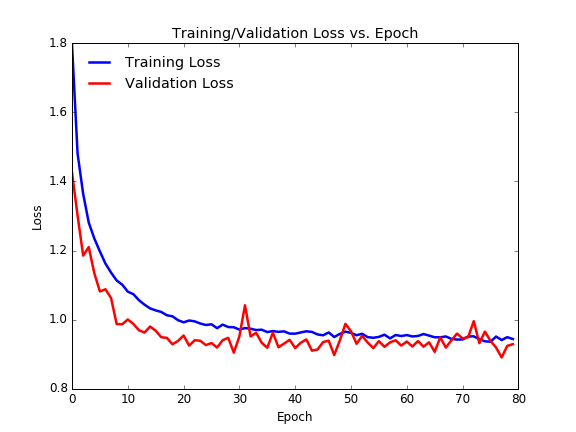
\includegraphics[width=1\linewidth]{baseline_loss.png}
  	\footnotesize{(a)}
 \end{minipage}\hfill%
\centering
 \begin{minipage}{.5\columnwidth}
\centering
  	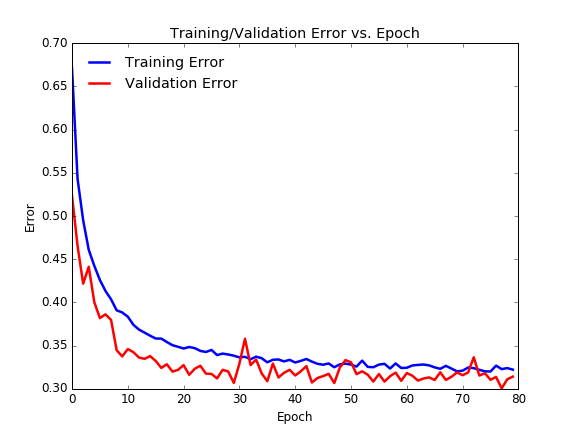
\includegraphics[width=1\columnwidth]{baseline_error.png}
  	\footnotesize{(b)}
 \end{minipage}\hfill%
\caption{Before question 1 and before doing anything. (a) Training and validation loss. (b) Training and validation error.}
\label{fig:baseline}
\end{figure}

\begin{figure}
\centering
\centering
 \begin{minipage}{.5\columnwidth}
\centering
  	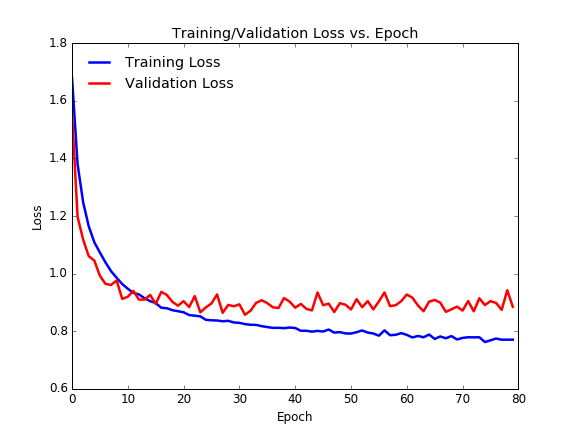
\includegraphics[width=1\linewidth]{question1_loss.png}
  	\footnotesize{(a)}
 \end{minipage}\hfill%
\centering
 \begin{minipage}{.5\columnwidth}
\centering
  	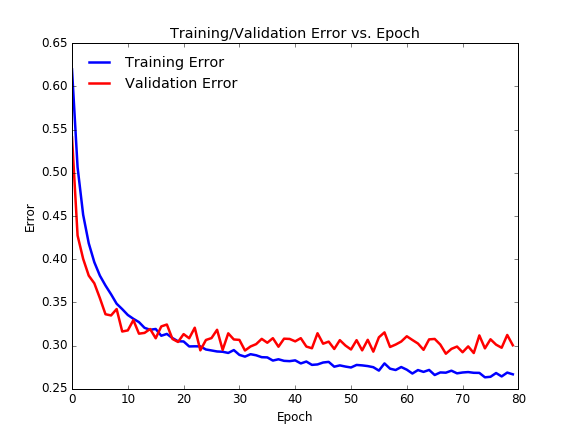
\includegraphics[width=1\columnwidth]{question1_error.png}
  	\footnotesize{(b)}
 \end{minipage}\hfill%
\caption{Question 1: remove dropout layer. (a) Training and validation loss. (b) Training and validation error.}
\label{fig:question1}
\end{figure}

\section{Question 2}

{\small Load the model you saved at step 1 as initialization to the training. Add another fully connected layer with 512 filters at the end (10 points). Train and save the model.}\\

We loaded the model from step 1 as initialization.  We then removed the last fully connected layer--the one converting to the number of classes--and softmax layer.  We added another fully connected layer with 512 filters, then added back 10-node fully connected layer and softmax.  We did not add back the weights for the 10-node fully connected layer from step 1.  (We also experimented with adding weights back from step 1 but the results were similar.)

Figure \ref{fig:question2} shows the loss and error plots.  Interestingly, the training error is slightly better than the one from question 1 but the training curve is not as smooth as before.  In addition, the validation error is now chaotic and increasing.  We probably implemented the code correctly because the training curve is still reasonable.  One explanation is that the model is overfitting very early: there is a slight decrease in the validation loss at first but it then it increases.

\begin{figure}
\centering
\centering
 \begin{minipage}{.5\columnwidth}
\centering
  	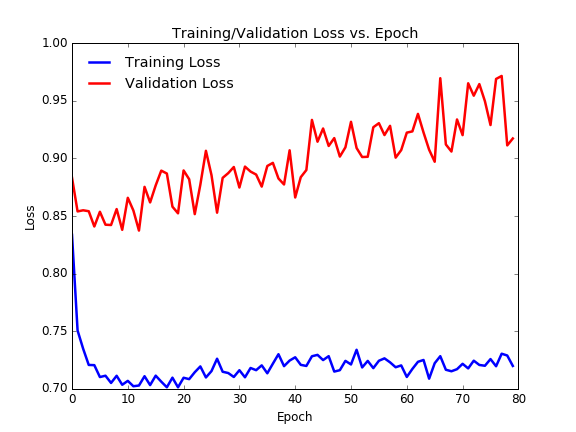
\includegraphics[width=1\linewidth]{question2_loss.png}
  	\footnotesize{(a)}
 \end{minipage}\hfill%
\centering
 \begin{minipage}{.5\columnwidth}
\centering
  	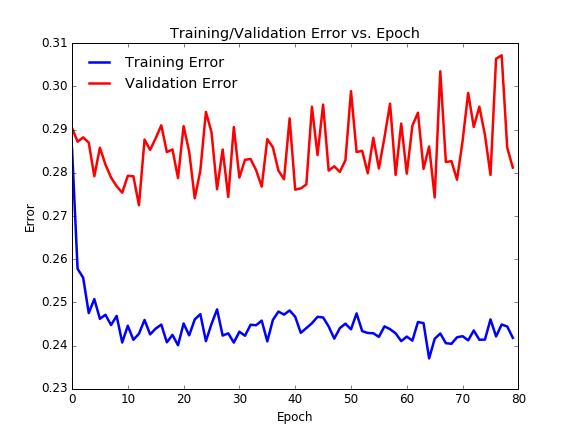
\includegraphics[width=1\columnwidth]{question2_error.png}
  	\footnotesize{(b)}
 \end{minipage}\hfill%
\caption{Question 2: add additional dense layer at the end. (a) Training and validation loss. (b) Training and validation error.}
\label{fig:question2}
\end{figure}

\section{Question 3}

{\small Load the model you saved at step 2 as initialization. Add dropout layers to both fully-connected layers (10 points), re-train the model. (Hint: in this case you may need to manually move the weights to the correct corresponding locations in the new model, but some has mentioned that you can "pop" a layer, so it might be easier than that).}\\

We loaded our mdoel from question 2 as initialization.  We added dropout layers after both fully-connected layers.

Figure \ref{fig:question3} shows the result after adding drop out back to all the fully connected layers.  The training and validation curves are higher than those in question 2.  The training curve still looks reasonable but the error is now around 0.45 at epoch 80 rather than around 0.24 from question 2.  The validation error, while still looking chaotic, is lower than the training error.  It would be reasonable that since dropout layers add regularization, the training performance would be worse at first.  We could also expect some ``chaotic'' behavior since we initialized the weights from question 2, which also had chaotic results.

\begin{figure}
\centering
\centering
 \begin{minipage}{.5\columnwidth}
\centering
  	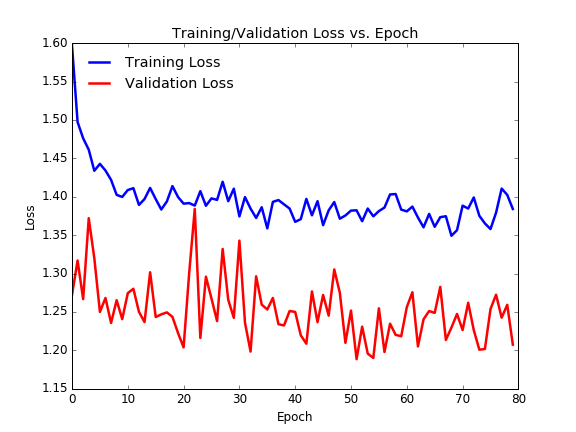
\includegraphics[width=1\linewidth]{question3_loss.png}
  	\footnotesize{(a)}
 \end{minipage}\hfill%
\centering
 \begin{minipage}{.5\columnwidth}
\centering
  	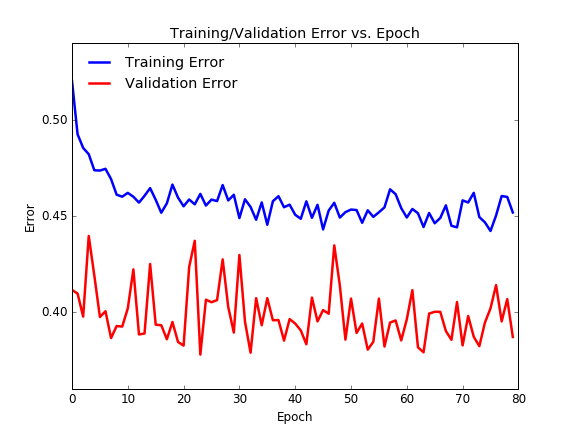
\includegraphics[width=1\columnwidth]{question3_error.png}
  	\footnotesize{(b)}
 \end{minipage}\hfill%
\caption{Question 3: add dropout after fully connected layers. (a) Training and validation loss. (b) Training and validation error.}
\label{fig:question3}
\end{figure}

\section{Question 4}

{\small Re-train the final model (after the model changes in tunings 1-3) from scratch. Try to use an adaptive schedule to tune the learning rate, you can choose from RMSprop, Adagrad and Adam (Hint: you don't need to implement any of these, look at Keras documentation please) (5 points).}\\

Figure \ref{fig:question4} shows the result of training 1-3 from scratch.  We trained with the Adam optimizer with the default settings.  We see a much nicer curve in contrast to the plots in question 3.  We see much better curves than from the previous questions.  It seems that training entirely from scratch is potentially better than fine-tuning the top layers, or at least fine-tuning in the sequence as prescribed by questions 1-3.  We also note that the performance is similar to the baseline.  Adding an extra layer does not help that much in this case.

\begin{figure}
\centering
\centering
 \begin{minipage}{.5\columnwidth}
\centering
  	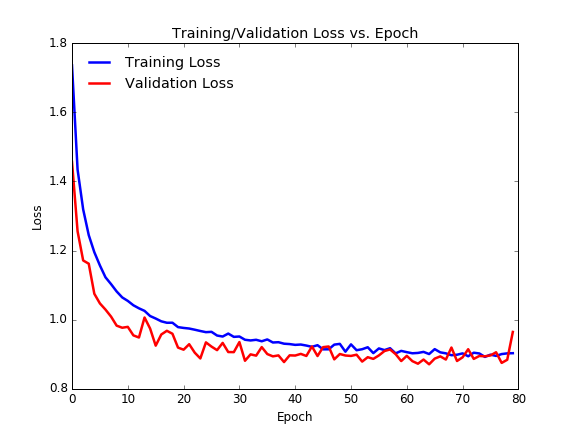
\includegraphics[width=1\linewidth]{question4_loss.png}
  	\footnotesize{(a)}
 \end{minipage}\hfill%
\centering
 \begin{minipage}{.5\columnwidth}
\centering
  	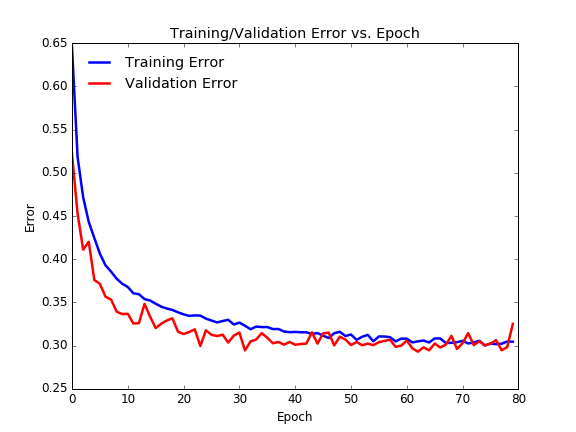
\includegraphics[width=1\columnwidth]{question4_error.png}
  	\footnotesize{(b)}
 \end{minipage}\hfill%
\caption{Question 4: train with changes 1-3 from scratch. (a) Training and validation loss. (b) Training and validation error.}
\label{fig:question4}
\end{figure}

\section{Question 5}

{\small Try to tune your network in two other ways (10 points) (e.g. add/remove a layer, change the activation function, add/remove regularizer, change the number of hidden units) not described in the previous four. You can start from random initializations or previous results as you wish.}\\

We explore two modifications. The first modification is to add more convolutional layers.  Specifically, instead of two $3 \times 3$ convolutional layers with $32$ filters, we add a third one before the first max pooling.  We also add another $3 \times 3$ convolutional layer with $64$ filters before the second max pooling layer.  This is the first modification.  The second modification is to simply modify question 4 such that all the fully connected layers contain 256 hidden nodes rather than 512.

Figure \ref{fig:question5a} shows the result of adding more convolutional layers.  Compared to the baseline, it seems to perform slightly worse.  This probably makes sense since from question 4, adding another dense layer did not help.  Perhaps removing layers would have been a better experiment.

Figure \ref{fig:question5b} shows the result of using 256 hidden nodes instead of 512 hidden nodes.  The training error is worse than the baseline but the validation error is about the same.  In this case, making the model more restrictive gave slightly worse results.  Thus model flexibility needs to be explored.

\begin{figure}
\centering
\centering
 \begin{minipage}{.5\columnwidth}
\centering
  	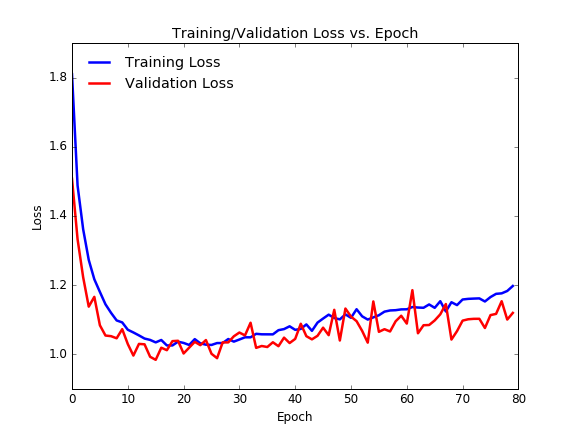
\includegraphics[width=1\linewidth]{question5a_loss.png}
  	\footnotesize{(a)}
 \end{minipage}\hfill%
\centering
 \begin{minipage}{.5\columnwidth}
\centering
  	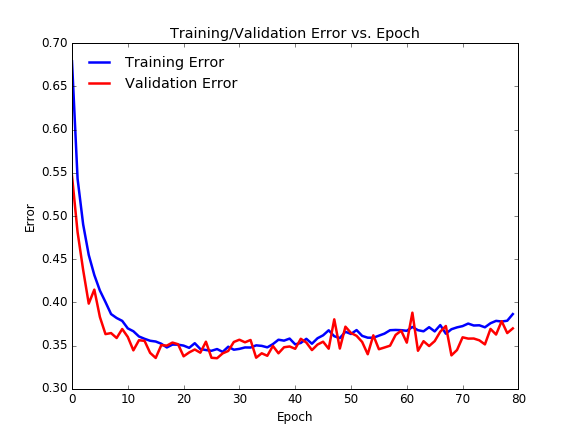
\includegraphics[width=1\columnwidth]{question5a_error.png}
  	\footnotesize{(b)}
 \end{minipage}\hfill%
\caption{Question 5: add more convolutional layers. (a) Training and validation loss. (b) Training and validation error.}
\label{fig:question5a}
\end{figure}

\begin{figure}
\centering
\centering
 \begin{minipage}{.5\columnwidth}
\centering
  	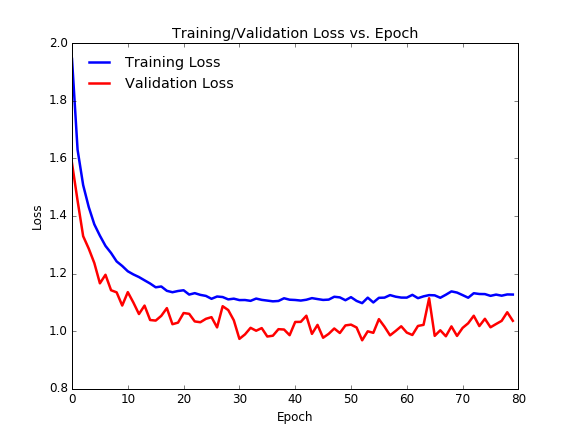
\includegraphics[width=1\linewidth]{question5b_loss.png}
  	\footnotesize{(a)}
 \end{minipage}\hfill%
\centering
 \begin{minipage}{.5\columnwidth}
\centering
  	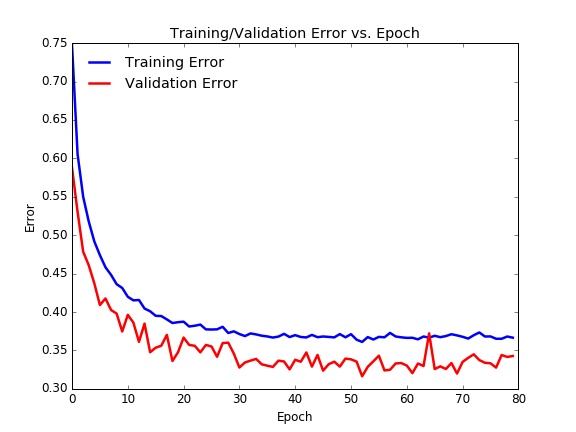
\includegraphics[width=1\columnwidth]{question5b_error.png}
  	\footnotesize{(b)}
 \end{minipage}\hfill%
\caption{Question 5: change dense layers of question 4 to 256 hidden units. (a) Training and validation loss. (b) Training and validation error.}
\label{fig:question5b}
\end{figure}

\end{document}
